% ==============================================
% ELEMENTOS PÓS-TEXTUAIS
% ==============================================
\postextual
% ||||||||||||||||||||||||||||||||||||||||||||||
% REFERÊNCIAS BIBLIOGRÁFICAS
% ||||||||||||||||||||||||||||||||||||||||||||||
%\bibliography{bibfile2}
% bibliografia john
\bibliography{ref-bibliografica}
% ----------------------------------------------
% Glossário
% ----------------------------------------------
% Consulte o manual da classe abntex2 para orientações sobre o glossário.
%
%\glossary
% ||||||||||||||||||||||||||||||||||||||||||||||
% APÊNDICES
% ||||||||||||||||||||||||||||||||||||||||||||||
\begin{apendicesenv}
% Imprime uma página indicando o início dos apêndices
\partapendices
% ----------------------------------------------
% Apêndice
% ----------------------------------------------
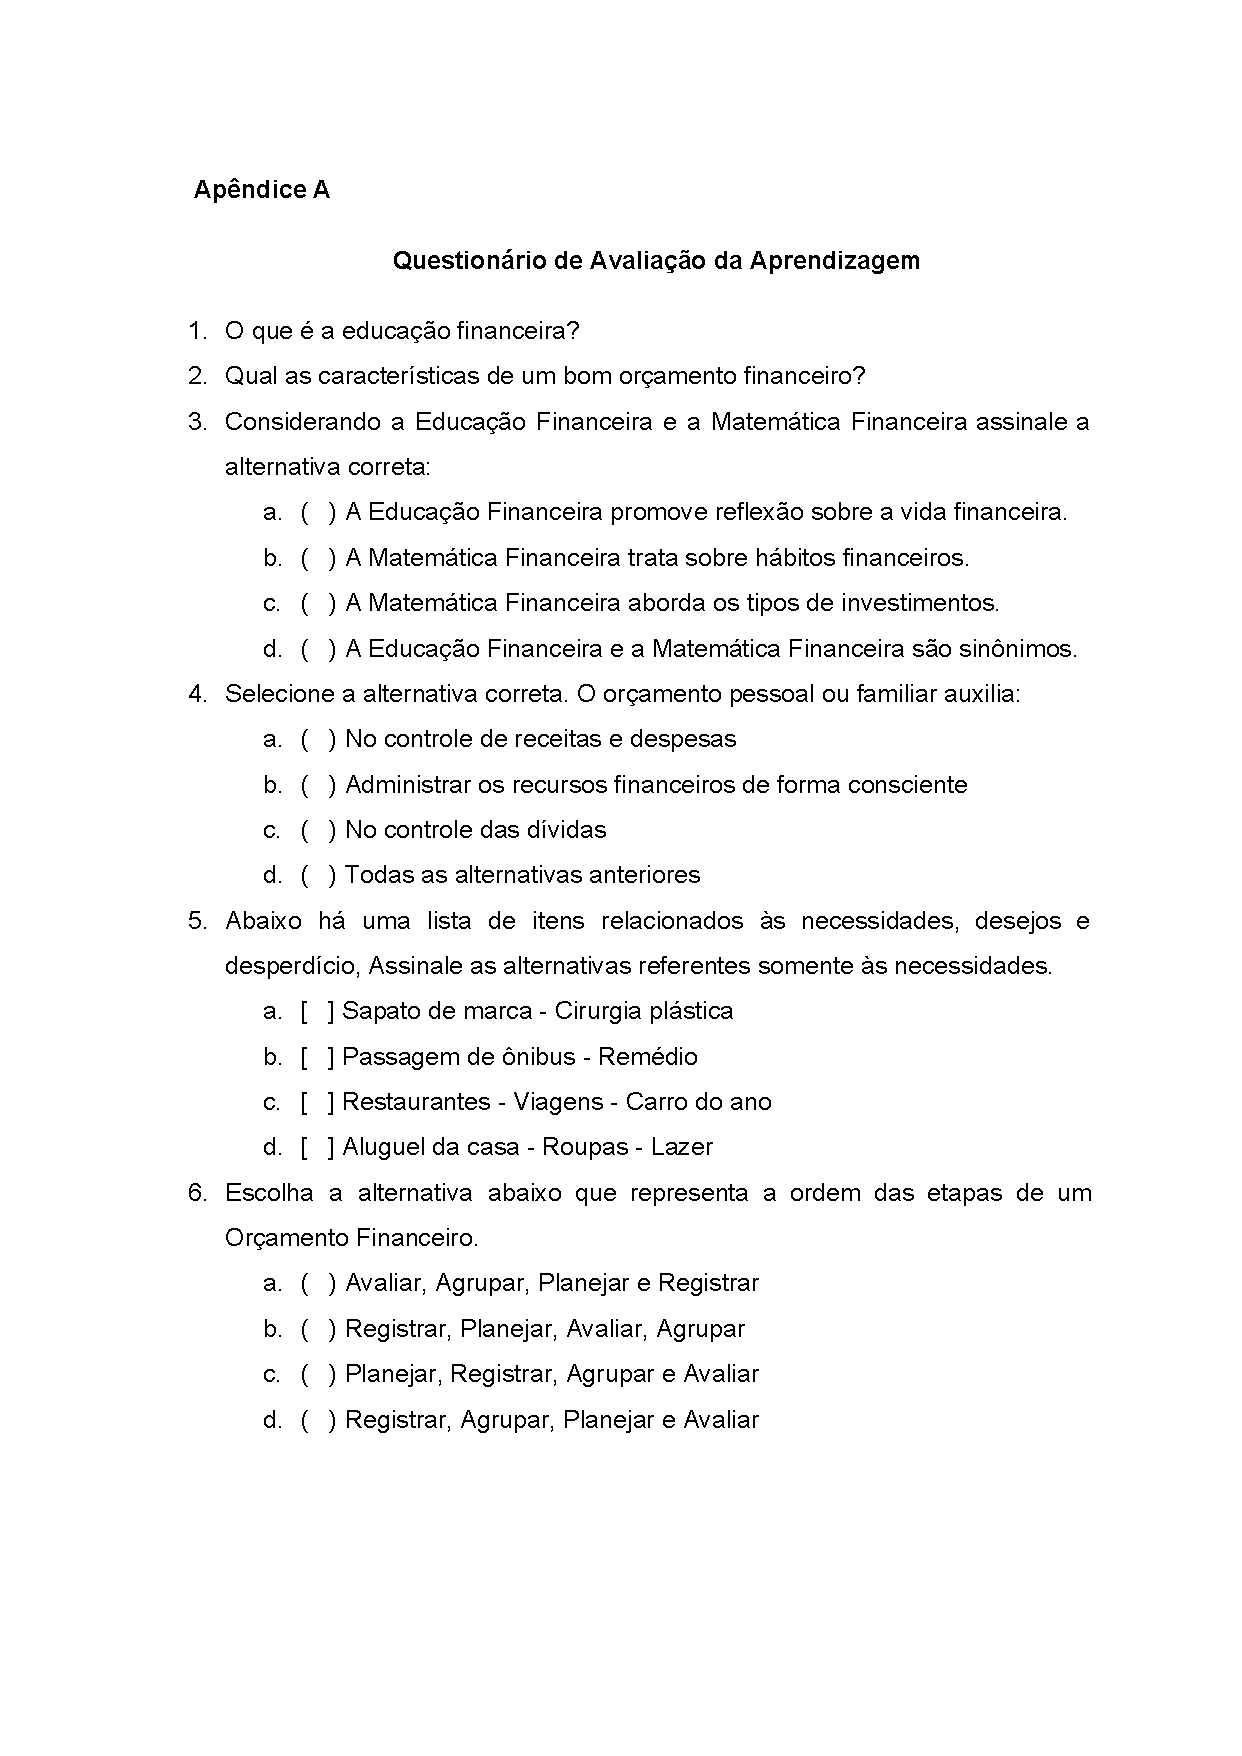
\includepdf[pages=-]{apendices/apendice-a_questionario-de-avaliacao-de-aprendizagem.pdf}
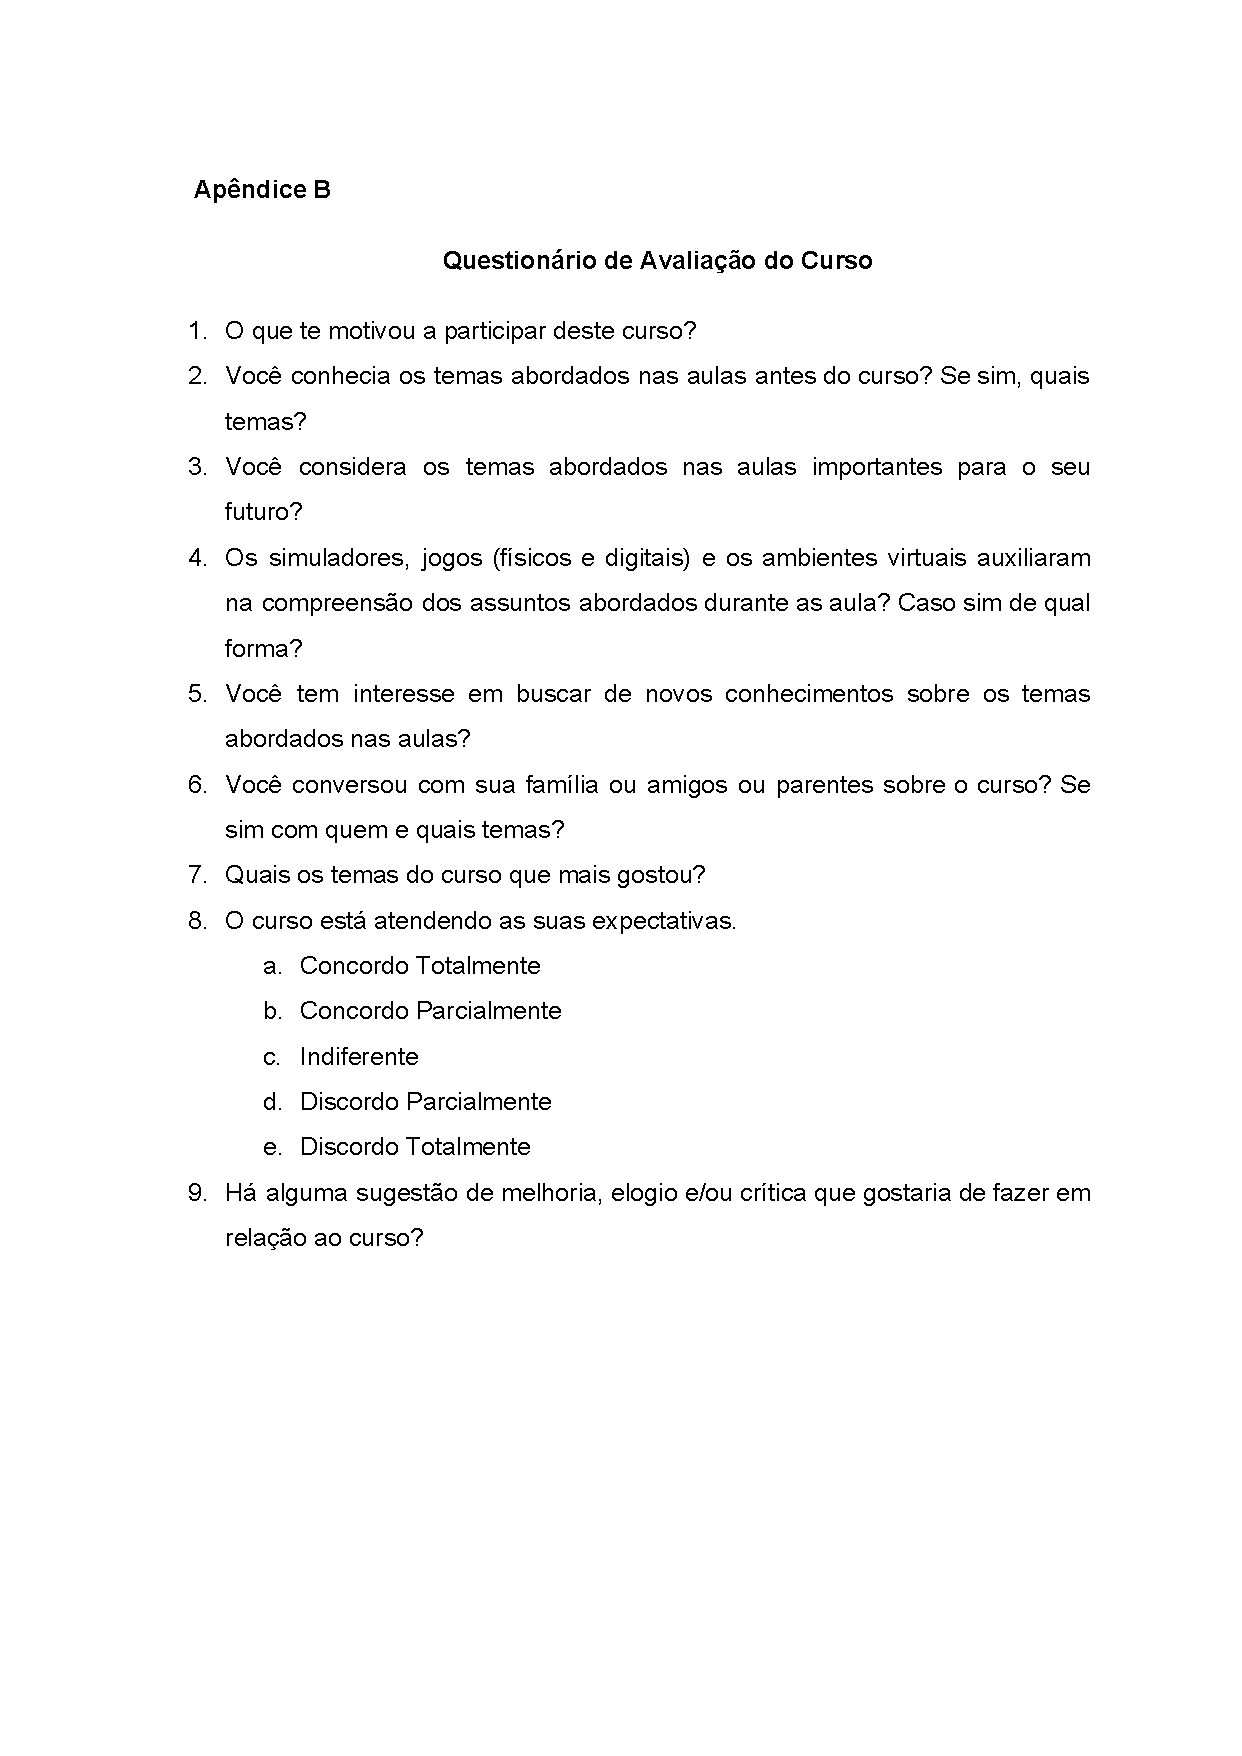
\includepdf[pages=-]{apendices/apendice-b_questionario-de-avaliacao-do-curso.pdf}
\end{apendicesenv}
% ||||||||||||||||||||||||||||||||||||||||||||||
% ANEXOS
% ||||||||||||||||||||||||||||||||||||||||||||||
%\begin{anexosenv}
% Imprime uma página indicando o início dos anexos
%\partanexos
% ----------------------------------------------
% Anexo 1
% ----------------------------------------------
%\chapter{Datasheet}\label{anexo1}
%\includepdf[pages=-]{pdfs/Datasheet.pdf}
% ----------------------------------------------
% Anexo 2
% ----------------------------------------------
%\chapter{Anexo 2}
%\end{anexosenv}
% ==============================================
% INDICE REMISSIVO
% ==============================================
\phantompart
\printindex
% ----------------------------------------------
% ||||||||||||||||||||||||||||||||||||||||||||||
% DOCUMENTO PARA ENTREGA VERSÃO FINAL
%||||||||||||||||||||||||||||||||||||||||||||||
\begin{comment}

\clearpage\thispagestyle{empty}\addtocounter{page}{-1}
\section*{ENTREGA DA VERSÃO FINAL DE DISSERTAÇÃO}

\vspace*{2cm}
Eu, \textsc{\imprimirorientador}, autorizo o aluno(a) \textsc{\imprimirautor} a entregar a versão final da dissertação de mestrado, à secretaria do MPIE, que foi por mim analisada e está de acordo com os apontamentos feitos pelos membros da banca de apresentação do referido aluno.

\vspace*{1cm}
\begin{center}   
   \assinatura{{\imprimirorientador} \\ Orientador}
\end{center}

\vspace*{1cm}
\begin{flushright}
	\imprimirlocal, 11 de Julho de \imprimirdata.
\end{flushright}
\clearpage
\end{comment}
